\documentclass[10pt,aspectratio=169]{beamer}
\usetheme{default}

\IfFileExists{lmodern.sty}{\usepackage{lmodern}}{}
\usepackage{booktabs}
\usepackage{multirow}
\usepackage{array}
\usepackage{colortbl}
\usepackage{appendixnumberbeamer}
\usepackage{listings}
\usepackage{amsmath}
\usepackage{tikz}
\usetikzlibrary{arrows.meta,positioning,calc,fit,backgrounds,shapes.misc}

\definecolor{dblue}{HTML}{3A3A3A}
\definecolor{accent}{HTML}{B61918}
\definecolor{okgreen}{HTML}{2E8B22}
% verdict colours, same as in the verdicts chart
\definecolor{vAccepted}{HTML}{2E8B22}
\definecolor{vNoSpeedup}{HTML}{E8A200}
\definecolor{vCuts}{HTML}{E14B4B}
\definecolor{vUnsat}{HTML}{3B3BBF}
\definecolor{vSyntax}{HTML}{F07EB0}
\definecolor{lightbg}{HTML}{F2F2F2}
\definecolor{midgray}{HTML}{8A8A8A}

\setbeamercolor{normal text}{fg=black,bg=white}
\setbeamercolor{structure}{fg=dblue}
\setbeamercolor{frametitle}{fg=black}
\setbeamercolor{title}{fg=black}
\setbeamercolor{alerted text}{fg=accent}
\setbeamercolor{block title}{fg=black,bg=lightbg!85!black}
\setbeamercolor{block body}{bg=lightbg}
\setbeamercolor{block title alerted}{fg=accent,bg=lightbg!85!black}
\setbeamercolor{block body alerted}{bg=lightbg}
\setbeamercolor{block title example}{fg=black,bg=lightbg!85!black}
\setbeamercolor{block body example}{bg=lightbg}
\setbeamertemplate{blocks}[rounded][shadow=false]
\setbeamertemplate{navigation symbols}{}
\setbeamertemplate{itemize items}{\small\raisebox{0.15ex}{\textbullet}}
\setbeamertemplate{enumerate items}[default]
\setbeamerfont{frametitle}{size=\Large,series=\bfseries}
\setbeamerfont{block title}{size=\normalsize,series=\bfseries}

\setbeamertemplate{frametitle}{%
  \vskip0.6em
  \begin{beamercolorbox}[wd=\paperwidth,leftskip=1.1em,rightskip=1.1em]{frametitle}%
    \usebeamerfont{frametitle}\strut\insertframetitle\hfill
    \raisebox{-0.1em}{\includegraphics[height=1.05em]{logo_unical.png}}%
  \end{beamercolorbox}%
  \vskip0.15em
  \begin{beamercolorbox}[wd=\paperwidth,leftskip=1.1em,rightskip=1.1em]{}%
    {\color{midgray!60}\rule{\dimexpr\paperwidth-2.2em\relax}{0.4pt}}%
  \end{beamercolorbox}%
  \vskip0.2em
}
\setbeamertemplate{footline}{%
  \usebeamerfont{footline}\scriptsize\color{midgray}%
  \hspace*{1.1em}\insertshortauthor\hfill\insertshorttitle\hfill
  \insertframenumber/\inserttotalframenumber\hspace*{1.1em}\vskip0.6em}

\setbeamertemplate{title page}{%
  \centering
  \includegraphics[height=1.4cm]{logo_unical.png}\par\vspace{1.4em}
  {\usebeamerfont{title}\Large\bfseries\inserttitle\par}
  \vspace{1.2em}
  {\color{midgray!60}\rule{0.5\textwidth}{0.4pt}}\par\vspace{1.0em}
  {\normalsize\insertauthor\par}\vspace{0.6em}
  {\small\color{dblue}\insertinstitute\par}\vspace{1.2em}
  {\small\insertdate\par}
}

\lstset{
  basicstyle=\ttfamily\footnotesize,
  breaklines=true,
  columns=fullflexible,
  keepspaces=true,
  showstringspaces=false,
  commentstyle=\color{gray}\itshape,
  morecomment=[l]{\%},
  frame=none,
  backgroundcolor=\color{lightbg},
  xleftmargin=3pt,xrightmargin=3pt,
  aboveskip=3pt,belowskip=3pt
}
\newcommand{\clingo}{\textsc{clingo}}
\newcommand{\verdict}[2]{\tikz[baseline=(v.base)]\node[fill=#1,text=white,rounded corners=2pt,inner sep=2pt,font=\scriptsize\bfseries](v){#2};}

\title[LLM-Generated Streamliners for ASP Optimization]{Generating Streamliners for ASP Optimization Problems\\with Large Language Models}
\author[\underline{M.~Duca}, I.~Frandina, F.~Ricca]{\underline{Marco Duca} \and Ilaria Frandina \and Francesco Ricca}
\institute{Department of Mathematics and Computer Science (DeMaCS)\\University of Calabria, Rende, Italy}
\date{TAASP 2026}

\begin{document}

\begin{frame}[plain]\titlepage\end{frame}

\begin{frame}{Introduction}
\begin{itemize}\setlength{\itemsep}{5pt}
\item Answer Set Programming (ASP) is a declarative programming paradigm for Knowledge Representation and reasoning.    
\item A \textbf{streamliner} is an auxiliary constraint that aims to reduce search effort of the solver.
\item Effective streamliners are usually \textbf{hand-crafted} by domain experts.
\item Large Language Models (LLMs) have recently been used to automatically generate streamliners for ASP \textbf{decision problems}.
\item \alert{Can LLM-generated streamliners speed up optimality proofs in ASP optimization problems?}
\end{itemize}
\end{frame}

% \begin{frame}[fragile]{Background: ASP Optimization}
% \begin{columns}[c,onlytextwidth]
% \column{0.55\textwidth}
% \begin{itemize}\setlength{\itemsep}{6pt}
% \item An ASP optimization problem searches for a stable model with the best value of a given objective, expressed as weak constraints.
% \item Weak constraints assigning costs to stable models without excluding them.
% \item To prove optimality, the solver must establish that no stable model with a better objective value exists.
% \end{itemize}
% \column{0.40\textwidth}
% \begin{block}{Example: Maximum Clique}
% \begin{lstlisting}[literate={~}{{$\sim$}}1]
% :~ nonClique(X). [1@0, X]
% \end{lstlisting}
% \small
% Each node excluded from the clique incurs a penalty of 1.
% Minimizing this penalty is equivalent to maximizing the clique size.
% \end{block}
% \end{columns}
% \end{frame}


% \begin{frame}{Background: Streamliners}
% \begin{itemize}\setlength{\itemsep}{5pt}
% \item A \alert{streamliner} is an auxiliary constraint added to an encoding.
% \item By ruling out alternatives that the solver would otherwise explore, streamliners can reduce search effort and improve solving time.
% \item \emph{Implied constraints} preserve all solutions, while \emph{symmetry-breaking constraints} eliminate equivalent ones, retaining at least one representative per symmetry class.
% \item In general, a streamliner may discard valid solutions and can even make a satisfiable instance unsatisfiable.
% \item Correctness can be guaranteed through a theoretical proof or checked empirically on a finite set of instances.
% \end{itemize}
% \end{frame}


\begin{frame}{Related work}
\begin{columns}[c,onlytextwidth]
\column{0.55\textwidth}
\begin{itemize}\setlength{\itemsep}{6pt}
% \item Gomes and Sellmann introduced streamliners in Constraint Programming (CP).
\item Spracklen et al. automated candidate generation through syntactic templates and empirical evaluation.
\item In \textsc{StreamLLM}, Voboril et al. replaced templates with constraints proposed by an LLM.
\item In \emph{Streamliners for Answer Set Programming} (ICLP 2026), Voboril et al. adapted LLM-based streamlining to ASP \alert{decision problems}.
\item The Virtual Best Encoding achieved PAR2 reductions of 47\% to 79\% across three decision benchmarks.
\end{itemize}
\column{0.40\textwidth}
\centering
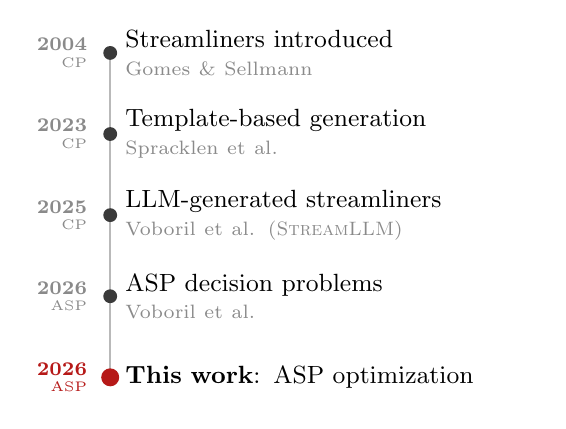
\begin{tikzpicture}[
  dot/.style={circle,fill=dblue,inner sep=0pt,minimum size=5pt},
  year/.style={font=\scriptsize,text=midgray,anchor=east,align=right},
  item/.style={font=\small,anchor=west,align=left,text width=5.2cm,inner sep=1pt}
]
\def\step{1.03}
\draw[midgray!60,line width=0.8pt] (0,0) -- (0,-4*\step);
\node[dot] at (0,0) {};
\node[year] at (-0.17,0) {\textbf{2004}\\[-2pt]{\tiny CP}};
\node[item] at (0.15,0) {Streamliners introduced\\[-1pt]{\scriptsize\color{midgray}Gomes \& Sellmann}};
\node[dot] at (0,-\step) {};
\node[year] at (-0.17,-\step) {\textbf{2023}\\[-2pt]{\tiny CP}};
\node[item] at (0.15,-\step) {\alert{Template}-based generation\\[-1pt]{\scriptsize\color{midgray}Spracklen et al.}};
\node[dot] at (0,-2*\step) {};
\node[year] at (-0.17,-2*\step) {\textbf{2025}\\[-2pt]{\tiny CP}};
\node[item] at (0.15,-2*\step) {LLM-generated streamliners\\[-1pt]{\scriptsize\color{midgray}Voboril et al. (\textsc{StreamLLM})}};
\node[dot] at (0,-3*\step) {};
\node[year] at (-0.17,-3*\step) {\textbf{2026}\\[-2pt]{\tiny ASP}};
\node[item] at (0.15,-3*\step) {ASP \alert{decision} problems\\[-1pt]{\scriptsize\color{midgray}Voboril et al.}};
\node[circle,fill=accent,inner sep=0pt,minimum size=6.5pt] at (0,-4*\step) {};
\node[year,text=accent] at (-0.17,-4*\step) {\textbf{2026}\\[-2pt]{\tiny ASP}};
\node[item] at (0.15,-4*\step) {\textbf{This work}: ASP \alert{optimization}};
\end{tikzpicture}
\end{columns}
\end{frame}

% \begin{frame}{Related work: Streamliners in ASP}
% \begin{columns}[c,onlytextwidth]
% \column{0.55\textwidth}
% \begin{itemize}\setlength{\itemsep}{6pt}
% \item In ASP, previous work on automated search-space reduction has largely focused on symmetry breaking.
% \item Tarzariol et al. used Inductive Logic Programming to learn reusable first-order symmetry-breaking constraints.
% \item In \emph{Streamliners for Answer Set Programming} (ICLP 2026), Voboril et al. adapted LLM-based streamlining to ASP \alert{decision problems}.
% \item The Virtual Best Encoding achieved PAR2 reductions of 47\% to 79\% across three decision benchmarks.
% \end{itemize}
% \column{0.40\textwidth}
% \centering
% \begin{tikzpicture}[
%   dot/.style={circle,fill=dblue,inner sep=0pt,minimum size=5pt},
%   year/.style={font=\scriptsize,text=midgray,anchor=east,align=right},
%   item/.style={font=\small,anchor=west,align=left,text width=5.2cm,inner sep=1pt}
% ]
% \def\step{1.03}
% \draw[midgray!60,line width=0.8pt] (0,0) -- (0,-4*\step);
% \node[dot] at (0,0) {};
% \node[year] at (-0.17,0) {\textbf{2004}\\[-2pt]{\tiny CP}};
% \node[item] at (0.15,0) {Streamliners introduced\\[-1pt]{\scriptsize\color{midgray}Gomes \& Sellmann}};
% \node[dot] at (0,-\step) {};
% \node[year] at (-0.17,-\step) {\textbf{2023}\\[-2pt]{\tiny CP}};
% \node[item] at (0.15,-\step) {\alert{Template}-based generation\\[-1pt]{\scriptsize\color{midgray}Spracklen et al.}};
% \node[dot] at (0,-2*\step) {};
% \node[year] at (-0.17,-2*\step) {\textbf{2025}\\[-2pt]{\tiny CP}};
% \node[item] at (0.15,-2*\step) {LLM-generated streamliners\\[-1pt]{\scriptsize\color{midgray}Voboril et al. (\textsc{StreamLLM})}};
% \node[dot] at (0,-3*\step) {};
% \node[year] at (-0.17,-3*\step) {\textbf{2026}\\[-2pt]{\tiny ASP}};
% \node[item] at (0.15,-3*\step) {ASP \alert{decision} problems\\[-1pt]{\scriptsize\color{midgray}Voboril et al.}};
% \node[circle,fill=accent,inner sep=0pt,minimum size=6.5pt] at (0,-4*\step) {};
% \node[year,text=accent] at (-0.17,-4*\step) {\textbf{2026}\\[-2pt]{\tiny ASP}};
% \node[item] at (0.15,-4*\step) {\textbf{This work}: ASP \alert{optimization}};
% \end{tikzpicture}
% \end{columns}
% \end{frame}

% \begin{frame}{Research Question}
% \begin{center}
%     \emph{Can LLM-generated streamliners speed up optimality proofs in ASP optimization problems?}
% \end{center}
% \end{frame}

% \begin{frame}{Related work (todo)}
% \begin{columns}[c,onlytextwidth]
% \column{0.42\textwidth}
% \begin{itemize}\setlength{\itemsep}{5pt}
%   \item Something
%   \item explaining
%   \item related
%   \item work.
% \end{itemize}
% \column{0.55\textwidth}
% \begin{tikzpicture}[
%   dot/.style={circle, fill=dblue, inner sep=0pt, minimum size=5pt},
%   year/.style={font=\scriptsize, text=midgray, anchor=east, align=right},
%   item/.style={font=\small, anchor=west, align=left, text width=6cm, inner sep=1pt}
% ]
% \def\step{1.05}
% \draw[midgray!60, line width=0.8pt] (0,0) -- (0,-4*\step);
% \node[dot] at (0,-0*\step) {};
% \node[year] at (-0.15,-0*\step) {\textbf{2004}\\[-2pt]{\tiny CP}};
% \node[item] at (0.15,-0*\step) {Streamliners introduced\\[-1pt]{\scriptsize\color{midgray}Gomes \& Sellmann}};
% \node[dot] at (0,-1*\step) {};
% \node[year] at (-0.15,-1*\step) {\textbf{2023}\\[-2pt]{\tiny CP}};
% \node[item] at (0.15,-1*\step) {Candidates from \alert{syntactic templates}\\[-1pt]{\scriptsize\color{midgray}Spracklen et al.}};
% \node[dot] at (0,-2*\step) {};
% \node[year] at (-0.15,-2*\step) {\textbf{2025}\\[-2pt]{\tiny CP}};
% \node[item] at (0.15,-2*\step) {\alert{LLM}-proposed candidates\\[-1pt]{\scriptsize\color{midgray}Voboril et al.\ (\textsc{StreamLLM})}};
% \node[dot] at (0,-3*\step) {};
% \node[year] at (-0.15,-3*\step) {\textbf{2026}\\[-2pt]{\tiny ASP}};
% \node[item] at (0.15,-3*\step) {LLM streamliners, \alert{decision} problems only\\[-1pt]{\scriptsize\color{midgray}Voboril et al.}};
% \node[circle, fill=accent, inner sep=0pt, minimum size=6.5pt] at (0,-4*\step) {};
% \node[year, text=accent] at (-0.15,-4*\step) {\textbf{2026}\\[-2pt]{\tiny ASP}};
% \node[item] at (0.15,-4*\step) {\textbf{This work}: LLM streamliners\\[-1pt]for \alert{optimization} problems};
% \end{tikzpicture}
% \end{columns}
% \end{frame}

 

\begin{frame}{From decision to optimization problems}
\begin{columns}[c,onlytextwidth]
\column{0.5\textwidth}
\begin{itemize}\setlength{\itemsep}{6pt}
\item For \textbf{decision problems}, a streamliner can fail by turning a satisfiable instance into an unsatisfiable one.
\item For \textbf{optimization problems}, it can also \alert{eliminate all optimal solutions}, while the solver still reports \texttt{OPTIMUM FOUND}.

\item Addressing these challenges requires a different approach to generate and evaluate streamliners.
\end{itemize}
% Moving from decision to optimization changes both how streamliners are \alert{evaluated} and how they can \alert{fail}.

% \begin{alertblock}{What changes with optimization problems}
% For decision problems, a streamliner fails only if the instance becomes UNSAT. 

% For optimization, restricting the search space could also \alert{cut all optimal solutions}, and the solver would still report \texttt{OPTIMUM FOUND}.
% \end{alertblock}
% We propose a pipeline in which each candidate is judged on the time to \alert{prove optimality}, checked against \alert{certified optimum}, and the outcome is fed back to the LLM.
\column{0.47\textwidth}
\centering
{\small\bfseries Example}\\[0.1em]
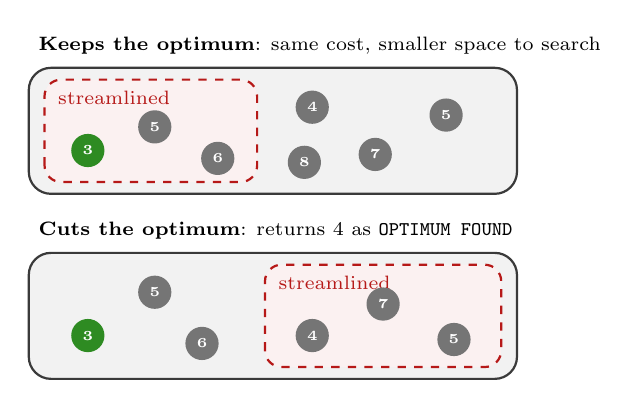
\begin{tikzpicture}[
  every node/.style={font=\scriptsize},
  sol/.style={circle,fill=dblue!70,inner sep=0pt,minimum size=12pt,text=white,font=\tiny\bfseries},
  opt/.style={circle,fill=okgreen,inner sep=0pt,minimum size=12pt,text=white,font=\tiny\bfseries},
  space/.style={draw=dblue,thick,fill=lightbg,rounded corners=8pt},
  region/.style={draw=accent,thick,dashed,rounded corners=6pt,fill=accent!6}
]
% ---------- (a) streamliner that keeps the optimum ----------
\node[anchor=south west,align=left] at (0,1.65) {\textbf{Keeps the optimum}: same cost, smaller space to search};
\draw[space] (0,0) rectangle (6.2,1.6);
\draw[region] (0.2,0.15) rectangle (2.9,1.45);
\node[accent,anchor=north west] at (0.25,1.43) {streamlined};
\node[opt] at (0.75,0.55) {3};
\node[sol] at (1.6,0.85) {5};
\node[sol] at (2.4,0.45) {6};
\node[sol] at (3.6,1.1) {4};
\node[sol] at (4.4,0.5) {7};
\node[sol] at (5.3,1.0) {5};
\node[sol] at (3.5,0.4) {8};
% ---------- (b) streamliner that cuts the optimum ----------
\begin{scope}[yshift=-2.35cm]
\node[anchor=south west,align=left] at (0,1.65) {\textbf{Cuts the optimum}: returns 4 as \texttt{OPTIMUM FOUND}};
\draw[space] (0,0) rectangle (6.2,1.6);
\draw[region] (3.0,0.15) rectangle (6.0,1.45);
\node[accent,anchor=north west] at (3.05,1.43) {streamlined};
\node[opt] at (0.75,0.55) {3};
\node[sol] at (1.6,1.1) {5};
\node[sol] at (2.2,0.45) {6};
\node[sol] at (3.6,0.55) {4};
\node[sol] at (4.5,0.95) {7};
\node[sol] at (5.4,0.5) {5};
\end{scope}
\end{tikzpicture}\\[0.4em]
{\scriptsize\color{midgray}each dot is a stable model, labelled by its cost}\\[0.4em]
\end{columns}
\end{frame}

\begin{frame}{The pipeline}
\centering
\scalebox{0.90}{%
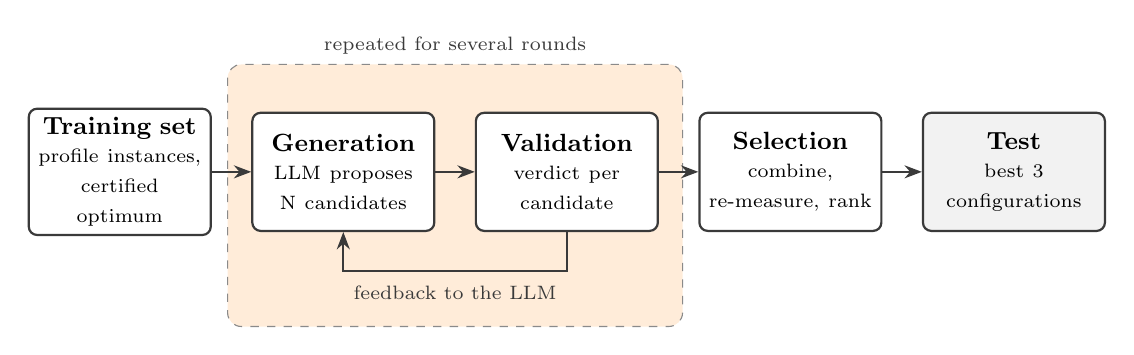
\begin{tikzpicture}[
  font=\small,
  box/.style={draw=dblue, fill=white, rounded corners=3pt, align=center,
    minimum height=15mm, text width=21mm, inner sep=3pt, line width=0.8pt},
  arr/.style={-{Stealth[length=2.2mm]}, thick, dblue},
  lab/.style={font=\scriptsize, align=center, dblue},
  node distance=5mm and 5mm
]
\node[box] (train) {\textbf{Training set}\\[2pt]\scriptsize profile instances,\\certified optimum};
\node[box, right=of train] (llm) {\textbf{Generation}\\[2pt]\scriptsize LLM proposes\\N candidates};
\node[box, right=of llm] (val) {\textbf{Validation}\\[2pt]\scriptsize verdict per\\candidate};
\node[box, right=of val] (sel) {\textbf{Selection}\\[2pt]\scriptsize combine,\\re-measure, rank};
\node[box, right=of sel, fill=lightbg] (test) {\textbf{Test}\\[2pt]\scriptsize best 3\\configurations};
\begin{scope}[on background layer]
\node[draw=midgray, dashed, rounded corners=5pt, fill=orange!15,
      inner xsep=3mm, inner ysep=9mm, yshift=-3mm, fit=(llm)(val),
      label={[font=\scriptsize, dblue]above:repeated for several rounds}] {};
\end{scope}
\draw[arr] (train) -- (llm);
\draw[arr] (llm) -- (val);
\draw[arr] (val.south) -- ++(0,-5mm) -| node[lab, below=0.5mm, pos=0.25]{feedback to the LLM} (llm.south);
\draw[arr] (val) -- (sel);
\draw[arr] (sel) -- (test);
\end{tikzpicture}
}
\begin{itemize}
\setlength{\itemsep}{5pt}
% \item The LLM proposes streamliner N candidates, each candidate is checked on the training set (against \alert{certified optimum}), and the outcome is reported back to the LLM.
\item Each candidate is judged on the time to \alert{prove optimality}, and checked against a \alert{certified optimum} from a Training Set.
\item Generation and validation are repeated over \alert{M rounds}: from the second one, the LLM is told how the previous candidates performed.
\item After the last round, the best candidates are applied to unseen test instances.
\end{itemize}
\end{frame}

%new per spiegazione formazione train
%new per spiegazione formazione train
\begin{frame}{Building the training set}
\begin{columns}[c,onlytextwidth]
\column{0.60\textwidth}
% \begin{itemize}\small\setlength{\itemsep}{7pt}
% \item Training instances must allow the original encoding to \alert{certify their optimum}, providing a reference value and certification time for evaluating candidates.
% \item They must also be challenging enough for performance differences to be distinguishable from \alert{measurement noise}.
% \item We profile the instances under a \alert{300\,s} budget, then select a small training set deterministically across three runtime classes.
% \item Very fast instances are used only for correctness validation, since their running times are too short for reliable speedup measurements.
% \end{itemize}

\begin{itemize}
    \item Training set stratified across \alert{three runtime classes}.
    
    \item Training instances must:
    \begin{itemize}
        \item have a \alert{certified optimum}, providing reference values and certification times.
        \item be \alert{challenging enough} to distinguish speedups from measurement noise.
    \end{itemize}

    \item Very fast instances are used only for correctness checks.
\end{itemize}

\column{0.40\textwidth}
\centering
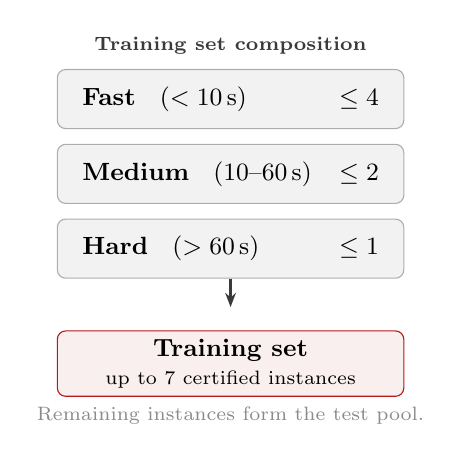
\begin{tikzpicture}[
  font=\small,
  tier/.style={draw=midgray!70, fill=lightbg, rounded corners=3pt,
    minimum width=4.4cm, minimum height=0.75cm, inner sep=3pt},
  arr/.style={-{Stealth[length=1.8mm]},dblue,thick}
]
\node[font=\scriptsize\bfseries,text=dblue] at (0,3.08)
  {Training set composition};
\node[tier] (fast) at (0,2.40) {};
\node[tier] (medium) at (0,1.45) {};
\node[tier] (hard) at (0,0.50) {};

\node[anchor=west,font=\small] at ([xshift=2mm]fast.west)
  {\textbf{Fast} \; ($<10$\,s)};
\node[anchor=east,font=\small] at ([xshift=-2mm]fast.east)
  {\alert{$\leq 4$}};
\node[anchor=west,font=\small] at ([xshift=2mm]medium.west)
  {\textbf{Medium} \; (10--60\,s)};
\node[anchor=east,font=\small] at ([xshift=-2mm]medium.east)
  {\alert{$\leq 2$}};
\node[anchor=west,font=\small] at ([xshift=2mm]hard.west)
  {\textbf{Hard} \; ($>60$\,s)};
\node[anchor=east,font=\small] at ([xshift=-2mm]hard.east)
  {\alert{$\leq 1$}};

\draw[arr] (hard.south) -- ++(0,-0.36);
\node[draw=accent,fill=accent!7,rounded corners=3pt,
  minimum width=4.4cm,minimum height=0.80cm,align=center,inner sep=3pt]
  (training) at (0,-0.96)
  {\textbf{Training set}\\[-1pt]{\scriptsize up to 7 certified instances}};
\node[font=\scriptsize,text=midgray] at (0,-1.62)
  {Remaining instances form the test pool.};
\end{tikzpicture}
\end{columns}
\end{frame}

%new per generazione e feedback
\begin{frame}{Generation and feedback}
\centering
\scalebox{0.75}{%
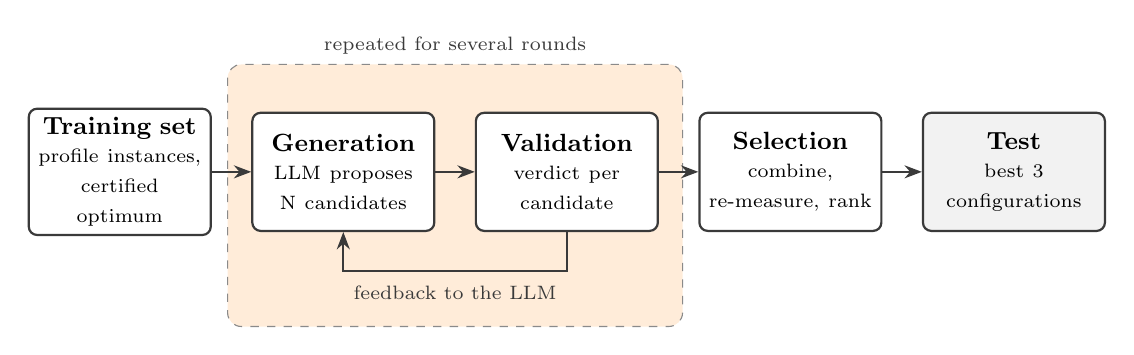
\begin{tikzpicture}[
  font=\small,
  box/.style={draw=dblue, fill=white, rounded corners=3pt, align=center,
    minimum height=15mm, text width=21mm, inner sep=3pt, line width=0.8pt},
  arr/.style={-{Stealth[length=2.2mm]}, thick, dblue},
  lab/.style={font=\scriptsize, align=center, dblue},
  node distance=5mm and 5mm
]
\node[box] (train) {\textbf{Training set}\\[2pt]\scriptsize profile instances,\\certified optimum};
\node[box, right=of train] (llm) {\textbf{Generation}\\[2pt]\scriptsize LLM proposes\\N candidates};
\node[box, right=of llm] (val) {\textbf{Validation}\\[2pt]\scriptsize verdict per\\candidate};
\node[box, right=of val] (sel) {\textbf{Selection}\\[2pt]\scriptsize combine,\\re-measure, rank};
\node[box, right=of sel, fill=lightbg] (test) {\textbf{Test}\\[2pt]\scriptsize best 3\\configurations};
\begin{scope}[on background layer]
\node[draw=midgray, dashed, rounded corners=5pt, fill=orange!15,
      inner xsep=3mm, inner ysep=9mm, yshift=-3mm, fit=(llm)(val),
      label={[font=\scriptsize, dblue]above:repeated for several rounds}] {};
\end{scope}
\draw[arr] (train) -- (llm);
\draw[arr] (llm) -- (val);
\draw[arr] (val.south) -- ++(0,-5mm) -| node[lab, below=0.5mm, pos=0.25]{feedback to the LLM} (llm.south);
\draw[arr] (val) -- (sel);
\draw[arr] (sel) -- (test);
\end{tikzpicture}
}
\begin{itemize}
    \item Each round, the LLM is asked to generate a set of \alert{candidate streamliners} in \clingo{} syntax.

    \item The prompt extends \textsc{StreamLLM} with:
    \begin{enumerate}
        \item focus on proving optimality, rather than
        finding a feasible solution;
        \item certified optima and proof times for training instances;
        \item guidance on constraint families useful for
        optimality proofs.
    \end{enumerate}

    \item \alert{Headed rules} are also retained and validated, despite requesting integrity constraints only.
    
    \item From round two, \alert{feedback} reports previous
    candidates and their validation verdicts.
    
\end{itemize}

\end{frame}

\begin{frame}{(Empirical) Validation and Selection}
\begin{columns}[T,onlytextwidth]
\column{0.52\textwidth}
\textbf{(Empirical) Validation}: check each candidate's \alert{solver outcome and cost} on every training instance; any failure rejects it.\\[0.25em]
\begin{tabular}{@{}ll@{}}
\verdict{vSyntax}{syntax-error} & \small parsing or grounding fails \\[1pt]
\verdict{vUnsat}{unsatisfiable} & \small an instance becomes UNSAT \\[1pt]
\verdict{vCuts}{cuts-optimum} & \small certified cost is worse
\end{tabular}
\vspace{0.4em}


Otherwise, compute \alert{certification-time speedups} $r_I$ on scored instances $T$, and aggregate into $G$:
\begingroup
\setlength{\abovedisplayskip}{3pt}
\setlength{\belowdisplayskip}{3pt}
\setlength{\abovedisplayshortskip}{3pt}
\setlength{\belowdisplayshortskip}{3pt}
\[
r_I = \frac{t_{\mathrm{orig}}(I)}{t_{\mathrm{cand}}(I)}
\qquad
G = \left(\prod_{I\in T} r_I\right)^{1/|T|}
\]
\endgroup
\begin{tabular}{@{}ll@{}}
\verdict{vNoSpeedup}{no-speedup} & \small $G < \theta$  \\[1pt]
\verdict{vAccepted}{accepted} & \small $G \ge \theta $
{\scriptsize\color{midgray}(retained over rounds)}
\end{tabular}
% Very fast instances are checked for correctness only. A timed-out
% instance contributes r_I = 0.5. Borderline G scores are re-measured.
\column{0.44\textwidth}
\textbf{Selection} then proceeds in four steps:\\[0.3em]
\begin{enumerate}\small
  \item Enumerate all subsets of $\le 3$ and rank them by VBE.
  \item Retain a small number of configurations.
  \item Each remaining configuration is run jointly to check for UNSAT.
  \item Configurations that pass this check are ranked by the running time of the joint run.
\end{enumerate}
\begin{block}{}
\centering The \textbf{3 best configurations} pass to the Test Phase.
\end{block}
\end{columns}
\end{frame}

\begin{frame}{Experimental setup}
\begin{columns}[T,onlytextwidth]
\column{0.38\textwidth}
\begin{itemize}
  \item \clingo{} 5.8, default branch-and-bound
  \item \textbf{Claude Opus 4.8} and \textbf{GPT-5.4}, 8 rounds $\times$ 5 candidates each
    \item Metric: \textbf{mean PAR2} over test instances;
uncertified runs count as twice the time budget.
\end{itemize}
\column{0.58\textwidth}
\textbf{Benchmarks} (4th ASP Competition, original encodings)\\[0.4em]
\footnotesize\setlength{\tabcolsep}{4pt}
\begin{tabular}{@{}llcccc@{}}
\toprule
 & & Train & Test & Budget & Pipeline \\
\midrule
\textbf{CM} & Crossing Minimization & 7 & 30 & 600\,s & 1--3\,h \\
\textbf{MC} & Maximum Clique & 7 & 30 & 600\,s & 1--2\,h \\
\textbf{SL} & Still Life & 5 & 21 & 1200\,s & 10--40\,min \\
\bottomrule
\end{tabular}\\[0.8em]
% {\normalsize\textbf{Computational cost}}\\[0.3em]
% {\footnotesize\raggedright
% A pipeline run takes one to three hours per LLM, mostly spent validating candidates on the training set. Profiling the dataset to choose the training instances is done \alert{once per benchmark}: a few hours on CM, mostly on instances that time out.\par}
\end{columns}
\end{frame}

% \begin{frame}{Experimental results: Overview}

% \centering
% \includegraphics[
%     width=0.90\textwidth,
%     height=0.60\textheight,
%     keepaspectratio
% ]{fig_verdicts.png}

% \begin{itemize}
%     \item The distribution of candidate verdicts varies across benchmarks. 
%     \item Crossing Minimization produces many \alert{accepted candidates}, while GPT-5.4 generates 14 candidates that \alert{cut the optimum} on Maximum Clique.
% \end{itemize}
% \end{frame}

% \begin{frame}{Preliminary run and revised pipeline}
% \begin{columns}[T,onlytextwidth]
% \column{0.49\textwidth}
% \footnotesize
% \textbf{First pipeline} (close to the decision-problem one): 8 easiest training instances, single measurement, sum of times, 6 rounds.
% \begin{itemize}\setlength{\itemsep}{1pt}
%   \item CM: already promising, PAR2 $-86\%$ to $-96\%$
%   \item MC: \alert{no measurable gain} ($0.98\times$--$1.10\times$)
% \end{itemize}
% \textbf{Diagnosis}
% \begin{itemize}\setlength{\itemsep}{1pt}
%   \item training $\le 22.5$\,s vs.\ test up to 293\,s: \alert{not representative}
%   \item runtime noise between repeated runs
%   \item \emph{accepted} used for both \alert{selection} and \alert{feedback}
% \end{itemize}
% \textbf{Fixes}: profiled training set, geometric mean and re-measurement, \alert{near misses} as feedback, 8 rounds.
% \column{0.48\textwidth}
% \centering
% \vspace{0.3em}
% \includegraphics[width=\linewidth]{fig_verdicts.png}\\[0.2em]
% \footnotesize Verdicts with the revised pipeline (40 per LLM).\\
% On MC, GPT-5.4 \alert{cuts the optimum} 14 times.
% \end{columns}
% \vspace{0.8em}
% {\footnotesize\color{midgray}Each final generation was run once. The preliminary run, with a different pipeline, already gave large gains on CM; a proper study of the variability across LLM runs is future work.\par}
% \end{frame}

% \begin{frame}[fragile]{Crossing Minimization}
% Order the nodes of a \textbf{layered graph} to \alert{minimize edge crossings}.
% \begin{columns}[T,onlytextwidth]
% \column{0.50\textwidth}
% \vspace{0.4em}
% {\footnotesize
% \textbf{Input} -- \texttt{in\_layer}, \texttt{width}, \texttt{edge}.\par\vspace{0.3em}
% \textbf{Guess/check} -- each node occupies exactly one position, distinct within its layer.\par\vspace{0.3em}
% \textbf{Optimize} -- derive the node ordering and penalize every crossing.\par}
% \vspace{0.15em}
% \begin{center}
% \begin{tikzpicture}[x=0.88cm,y=0.84cm,
%   every node/.style={font=\scriptsize},
%   v/.style={circle,draw=dblue,fill=lightbg,minimum size=5.5mm,inner sep=0pt}]
%   \node[v] (a) at (0,1.13) {A};
%   \node[v] (b) at (2.8,1.13) {B};
%   \node[v] (c) at (0,0) {C};
%   \node[v] (d) at (2.8,0) {D};
%   \draw[accent,thick] (a) -- (d);
%   \draw[accent,thick] (b) -- (c);
%   \fill[accent] (1.4,0.565) circle (1.8pt);
%   \node[above=2pt,text=midgray,font=\tiny] at (1.4,1.43) {Layer 1};
%   \node[below=2pt,text=midgray,font=\tiny] at (1.4,-0.28) {Layer 2};
% \end{tikzpicture}\\[-2pt]
% {\scriptsize\color{accent}One crossing}
% \end{center}
% \column{0.50\textwidth}
% \begin{center}
% \begin{lstlisting}[basicstyle=\ttfamily\fontsize{6.5}{6.65}\selectfont,
% aboveskip=2pt,belowskip=0pt,breaklines=false,literate={~}{{$\sim$}}1]
% % guess
% pvalue(L,0) :- width(L,_).
% pvalue(L,X+1) :- pvalue(L,X), width(L,T), X<T.
% position(N,P) | not_position(N,P) :-
%    in_layer(L,N), width(L,T), pvalue(L,Q), Q<T, P=Q+1.
% % check
% :- position(N,P1), position(N,P2), P1<P2.
% :- in_layer(L,A), in_layer(L,B), A!=B,
%    position(A,P), position(B,P).
% node_assigned_at_position(N) :- position(N,_).
% :- in_layer(L,N), not node_assigned_at_position(N).
% % optimization
% edge_from_same_layers(A,B,C,D) :-
%    edge(A,B), edge(C,D), A<C, B!=D,
%    in_layer(L,A), in_layer(L,C).
% antecedent(A,B) :- in_layer(L,A), in_layer(L,B),
%    A!=B, position(A,P), position(B,Q), P<Q.
% crossing(A,B,C,D) :- edge_from_same_layers(A,B,C,D),
%    antecedent(A,C), antecedent(D,B).
% crossing(A,B,C,D) :- edge_from_same_layers(A,B,C,D),
%    antecedent(C,A), antecedent(B,D).
% :~ crossing(A,B,C,D). [1@0,A,B,C,D]
% \end{lstlisting}
% \end{center}

% \end{columns}
% \end{frame}

\begin{frame}[fragile]{Experimental results: Crossing Minimization}
% The original encoding assigns a unique position to each node.
% Consequently any two distinct nodes in the same layer have exactly one order.
\vspace{0.22em}
\begin{columns}[T,onlytextwidth]
\column{0.55\textwidth}
{\footnotesize\bfseries\color{accent}C1 (Opus 4.8) -- derive the ordering}\par
\begin{lstlisting}[basicstyle=\ttfamily\fontsize{7.0}{7.5}\selectfont,breaklines=false,aboveskip=3pt,belowskip=3pt]
antecedent(N1,N2) :- in_layer(L,N1), in_layer(L,N2),
   N1 != N2, not antecedent(N2,N1),
   position(N1,_), position(N2,_).
\end{lstlisting}
{\footnotesize\raggedright
If \(N_2\) does \emph{not} precede \(N_1\), derive that \(N_1\)
precedes \(N_2\). Both nodes already have positions.\par}
\vspace{0.35em}
{\footnotesize\bfseries\color{accent}C3 (GPT-5.4) -- forbid an unordered pair}\par
\begin{lstlisting}[basicstyle=\ttfamily\fontsize{7.0}{7.5}\selectfont,breaklines=false,aboveskip=3pt,belowskip=3pt]
:- in_layer(L,N1), in_layer(L,N2), N1 < N2,
   not antecedent(N1,N2), not antecedent(N2,N1).
\end{lstlisting}
{\footnotesize\raggedright
Reject a pair if \emph{neither} node precedes the other.
\texttt{N1 < N2} avoids checking the same pair twice.\par}
\vspace{0.35em}
\begin{block}{Takeaway}
\footnotesize
Both rules restate an implied property, so \alert{no valid layout is removed}.
Explicit order information can strengthen propagation and accelerate
the \emph{proof of optimality}
\end{block}

\column{0.43\textwidth}
\centering
\includegraphics[width=0.65\linewidth]{fig_scatter_crossing.png}\\[-0.05em]
\vspace{0.25em}
{\centering\scriptsize
\setlength{\tabcolsep}{3.7pt}
\renewcommand{\arraystretch}{1.18}
\begin{tabular}{@{}lccc@{}}
\toprule
Encoding & Certified & PAR2 (s) & Reduction \\
\midrule
Original & 22/30 & 337.10 & --- \\
Opus (C1) & 30/30 & 2.02 & 99.4\% \\
\textbf{GPT (C3)} & \textbf{30/30} & \textbf{0.99} & \alert{\textbf{99.7\%}} \\
\bottomrule
\end{tabular}\par}
\vspace{0.15em}
{\scriptsize\color{midgray}Known optima matched: 22/22.}
\end{columns}
\end{frame}

%Not sure between this and the previous
% \begin{frame}[fragile]{(ALT) Experimental results: Crossing Minimization}
% \vspace*{-0.12em}
% {\footnotesize\textbf{Key observation.} Distinct node positions already imply \alert{exactly one ordering} for every pair in a layer.\par}
% \vspace{0.02em}
% \begin{columns}[T,onlytextwidth]
% \column{0.55\textwidth}
% {\footnotesize\bfseries\color{accent}C1 (Opus 4.8) -- derive the ordering}\par
% \begin{lstlisting}[basicstyle=\ttfamily\fontsize{6.8}{7.3}\selectfont,breaklines=false,aboveskip=2pt,belowskip=2pt]
% antecedent(N1,N2) :- in_layer(L,N1), in_layer(L,N2),
%    N1 != N2, not antecedent(N2,N1),
%    position(N1,_), position(N2,_).
% \end{lstlisting}
% {\footnotesize\raggedright
% If \(N_2\) does \emph{not} precede \(N_1\), derive that \(N_1\) precedes \(N_2\).\par}
% \vspace{0.25em}
% {\footnotesize\bfseries\color{accent}C3 (GPT-5.4) -- forbid an unordered pair}\par
% \begin{lstlisting}[basicstyle=\ttfamily\fontsize{6.8}{7.3}\selectfont,breaklines=false,aboveskip=2pt,belowskip=2pt]
% :- in_layer(L,N1), in_layer(L,N2), N1 < N2,
%    not antecedent(N1,N2), not antecedent(N2,N1).
% \end{lstlisting}
% {\footnotesize\raggedright
% Reject a pair if \emph{neither} node precedes the other;
% \texttt{N1 < N2} checks each pair once.\par}
% \vspace{0.23em}
% {\scriptsize\raggedright\textbf{Effect.} \alert{No solution is lost}; propagation helps prove optimality.\par}
% \vspace{0.12em}
% {\centering\fontsize{6.35}{7.1}\selectfont
% \setlength{\tabcolsep}{3.25pt}
% \renewcommand{\arraystretch}{1.0}
% \begin{tabular}{@{}llccc@{}}
% \toprule
% Encoding & Streaml. & Certified & PAR2 (s) & Reduction \\
% \midrule
% Original & --- & 22/30 & 10113.0 & --- \\
% Opus 1 & C1,C2 & 30/30 & 99.8 & 99.0\% \\
% Opus 2 & C1 & 30/30 & 60.6 & 99.4\% \\
% \textbf{GPT 1} & \textbf{C3} & \textbf{30/30} & \textbf{29.7} & \alert{\textbf{99.7\%}} \\
% GPT 2 & C3,C4 & 30/30 & 29.7 & 99.7\% \\
% GPT 3 & C3,C5 & 30/30 & 46.3 & 99.5\% \\
% \bottomrule
% \end{tabular}\par}
% \column{0.43\textwidth}
% \centering
% \vspace*{-0.18em}
% \includegraphics[height=5.48cm,keepaspectratio]{fig_scatter_crossing.png}\\[-0.15em]
% {\scriptsize\raggedright Below diagonal = faster; gains grow with difficulty.\par}
% {\scriptsize\raggedright Known optima matched: 22/22.\par}
% \end{columns}
% \end{frame}

% \begin{frame}[fragile]{Maximum Clique}
% Find the \alert{largest subset of nodes} in which \textbf{every pair is connected by an edge}
% \begin{columns}[T,onlytextwidth]
% \column{0.49\textwidth}
% \vspace{0.45em}
% {\footnotesize
% \textbf{Input} -- \texttt{node(X)}, \texttt{edge(X,Y)}: an undirected graph.\par\vspace{0.35em}
% % \textbf{Normalize} -- \texttt{uedge(X,Y)} stores each edge with its
% % \emph{smaller endpoint first}.\par\vspace{0.35em}
% \textbf{Guess/check} -- choose the clique; exclude a pair of
% non-adjacent nodes from being selected together.\par\vspace{0.35em}
% \textbf{Optimize} -- penalize every excluded node: minimizing
% exclusions \alert{maximizes clique size}.\par}
% \vspace{0.45em}
% \begin{center}
% \begin{tikzpicture}[x=0.80cm,y=0.73cm,
%  every node/.style={font=\scriptsize},
%  chosen/.style={circle,draw=accent,fill=accent,text=white,minimum size=6.7mm,inner sep=0pt},
%  other/.style={circle,draw=midgray,fill=lightbg,minimum size=6.7mm,inner sep=0pt}]
%  \node[chosen] (one) at (0.65,1.65) {1};
%  \node[chosen] (two) at (3.45,1.65) {2};
%  \node[chosen] (three) at (2.05,0.26) {3};
%  \node[other] (four) at (-0.3,0.30) {4};
%  \node[other] (five) at (4.4,0.30) {5};
%  \begin{scope}[on background layer]
%   \draw[accent,line width=1.5pt] (one)--(two)--(three)--(one);
%   \draw[midgray,line width=0.8pt] (one)--(four) (two)--(five) (three)--(five);
%  \end{scope}
%  \node[font=\scriptsize,text=accent] at (2.05,-0.50) {Clique \{1,2,3\} of size 3};
% \end{tikzpicture}
% \end{center}
% \column{0.50\textwidth}
% \begin{center}
% \begin{lstlisting}[basicstyle=\ttfamily\fontsize{7.6}{8.2}\selectfont,
%  aboveskip=2pt,belowskip=0pt,breaklines=false]
% % normalize: smaller node ID first
% uedge(X,Y) :- edge(X,Y), X < Y.
% uedge(Y,X) :- edge(X,Y), Y < X.

% % guess membership
% clique(X) | nonClique(X) :- node(X).

% % check: all chosen nodes are adjacent
% :- clique(X), clique(Y),
%    not uedge(X,Y), X < Y.

% % minimize excluded nodes
% :~ nonClique(X). [1@0,X]
% \end{lstlisting}
% \end{center}

% \end{columns}
% \end{frame}

\begin{frame}[fragile]{Experimental results: Maximum Clique}
% The original constraint forbids choosing two non-adjacent vertices.
% M1 and M3 explicitly encode the exclusion that must follow.
\vspace{0.22em}
\begin{columns}[T,onlytextwidth]
\column{0.55\textwidth}
{\footnotesize\bfseries\color{accent}M1 (Opus 4.8) -- derive an exclusion}\par
\begin{lstlisting}[basicstyle=\ttfamily\fontsize{7.0}{7.5}\selectfont,breaklines=false,aboveskip=3pt,belowskip=3pt]
nonClique(X) :- clique(Y), node(X), X > Y,
   not uedge(Y,X).
\end{lstlisting}
{\footnotesize\raggedright
If \(Y\) is in the clique but \(X\) is \emph{not adjacent} to \(Y\),
then \(X\) must be excluded.\par}
\vspace{0.35em}
{\footnotesize\bfseries\color{accent}M3 (GPT-5.4) -- require an exclusion}\par
\begin{lstlisting}[basicstyle=\ttfamily\fontsize{7.0}{7.5}\selectfont,breaklines=false,aboveskip=3pt,belowskip=3pt]
nonClique(X) | nonClique(Y) :- node(X), node(Y),
   X < Y, not uedge(X,Y).
\end{lstlisting}
{\footnotesize\raggedright
For any \emph{non-adjacent} pair, at least one node must be
excluded.\par}
\vspace{0.35em}
\alert{M3+M5 cut the optimum on 11/30 instances.}
\begin{block}{Takeaway}
\footnotesize
M1 and M3 make \alert{implied exclusions} explicit,
preserving all valid cliques while accelerating
the proof of optimality.
\end{block}
\column{0.43\textwidth}
\centering
\includegraphics[width=0.65\linewidth]{fig_scatter_maxclique.png}\\[-0.05em]
\vspace{0.25em}
{\centering\scriptsize
\setlength{\tabcolsep}{3.1pt}
\renewcommand{\arraystretch}{1.08}
\begin{tabular}{@{}lccc@{}}
\toprule
Encoding & Certified & PAR2 (s) & Reduction \\
\midrule
Original & 30/30 & 37.23 & --- \\
Opus (M1,M2) & 30/30 & 18.54 & 50.2\% \\
\textbf{GPT (M3)} & \textbf{30/30} & \textbf{8.79} & \alert{\textbf{76.4\%}} \\
\bottomrule
\end{tabular}\par}
\vspace{0.08em}
{\scriptsize\color{midgray}
Optima matched: 30/30 (both shown).}
\end{columns}
\end{frame}

% \begin{frame}[fragile]{Maximum Clique}
% \begin{columns}[T,onlytextwidth]
% \column{0.52\textwidth}
% \begin{lstlisting}[basicstyle=\ttfamily\scriptsize]
% % M1 (Opus 4.8)
% nonClique(X) :- clique(Y), node(X), X > Y,
%    not uedge(Y,X).
% % M3 (GPT-5.4)
% nonClique(X) | nonClique(Y) :- node(X), node(Y),
%    X < Y, not uedge(X,Y).
% \end{lstlisting}
% \vspace{0.6em}
% {\footnotesize\raggedright
% Both constraints say that, of two non-adjacent nodes, at least one stays out of the clique. This already follows from the clique property, but stating it lets the solver \alert{exclude nodes earlier}. In the preliminary run the gain was 5\%; now it is 76\%.\par}
% \vspace{0.6em}
% {\centering\scriptsize
% \setlength{\tabcolsep}{4pt}
% \begin{tabular}{@{}llcccr@{}}
% \toprule
% Enc. & Stream. & Certified & Opt.\ match & PAR2 & red. \\
% \midrule
% Original & --- & 30/30 & 30/30 & 1116.8 & --- \\
% Opus 1 & M1,M2 & 30/30 & 30/30 & 556.2 & 50.2\% \\
% Opus 2 & M1 & 30/30 & 30/30 & 578.3 & 48.2\% \\
% \textbf{GPT 1} & \textbf{M3} & 30/30 & 30/30 & \textbf{263.7} & \textbf{76.4\%} \\
% GPT 2 & M3,M4 & 30/30 & 30/30 & 359.6 & 67.8\% \\
% GPT 3 & M3,M5 & 30/30 & \alert{19/30} & 405.6 & 63.7\% \\
% \bottomrule
% \end{tabular}\par}
% \column{0.45\textwidth}
% \centering
% \includegraphics[width=0.80\linewidth]{fig_scatter_maxclique.png}\\[0.3em]
% \footnotesize Certification time per instance. M3 speedup\\ grows from \alert{$1.8\times$} (225 nodes) to \alert{$>7\times$} (largest).
% \end{columns}
% \end{frame}

% \begin{frame}[fragile]{A silent failure: M5 cuts the optimum}
% \begin{lstlisting}
% % M5 (GPT-5.4) -- intended: canonical choice between "twin" nodes
% :- clique(Y), nonClique(X), X < Y,
%    #count{Z: uedge(X,Z), Z != Y, not uedge(Y,Z)} = 0,
%    #count{Z: uedge(Y,Z), Z != X, not uedge(X,Z)} = 0.
% \end{lstlisting}
% \begin{columns}[T,onlytextwidth]
% \column{0.52\textwidth}
% \begin{itemize}
%   \item M5 tries to pick one of two \emph{twin} nodes, i.e.\ nodes with the same neighbours.
%   \item Since \texttt{uedge} stores the \alert{smaller endpoint first}, the counts only see neighbours with a higher index.
%   \item Some non-twin nodes are then treated as twins, and the constraint removes every optimal solution.
%   \item The pattern never occurs on the training instances, only on larger test ones.
% \end{itemize}
% \column{0.44\textwidth}
% \begin{alertblock}{Effect on \{M3, M5\}}
% Suboptimal on \textbf{11 of 30} instances: one node fewer than the maximum in 10 cases, two fewer in one.
% \end{alertblock}
% \small M5 entered selection only as a \emph{near miss} ($G = 1.15$). Configurations made of accepted candidates always matched the optimum.
% \end{columns}
% \end{frame}

% \begin{frame}[fragile]{Still Life}
% Find the \alert{largest stable, connected set of living cells} on an $N\times N$ Game of Life board.
% \begin{columns}[T,onlytextwidth]
% \column{0.45\textwidth}
% \vspace{0.28em}
% \begin{center}    
% {\raggedright
% \textbf{Guess} -- each interior cell may be alive or dead; the border is dead.\par\vspace{0.24em}
% \textbf{Stability} -- living cells have 2--3 live neighbours; dead cells must not have exactly 3.\par\vspace{0.24em}
% \textbf{Connectivity} -- every living cell must be reachable from one seed via neighbouring cells.\par\vspace{0.24em}
% \textbf{Optimize} -- minimize dead cells (equivalently \alert{maximize living cells}).\par}
% \end{center}
% % \vspace{0.22em}
% % \begin{center}
% % % \begin{tikzpicture}[x=0.34cm,y=0.34cm]
% % %   \foreach \x in {0,...,4} {\foreach \y in {0,...,4} {
% % %     \fill[lightbg] (\x,\y) rectangle ++(1,1);
% % %     \draw[midgray!60,line width=0.4pt] (\x,\y) rectangle ++(1,1);
% % %   }}
% % %   \foreach \x in {1,2} {\foreach \y in {1,2} {
% % %     \fill[accent] (\x+0.07,\y+0.07) rectangle ++(0.86,0.86);
% % %   }}
% % %   \node[font=\scriptsize,text=accent,anchor=west] at (5.2,3.25) {Living};
% % %   \fill[accent] (4.7,3.1) rectangle ++(0.35,0.35);
% % %   \node[font=\scriptsize,text=midgray,anchor=west] at (5.2,2.4) {Dead};
% % %   \draw[midgray] (4.7,2.25) rectangle ++(0.35,0.35);
% % % \end{tikzpicture}\\[-0.05em]
% % % {\scriptsize\color{midgray}Example: a connected, stable $2\times2$ block}
% % \end{center}
% \column{0.53\textwidth}
% \begin{center}
% \begin{lstlisting}[basicstyle=\ttfamily\fontsize{5.27}{5.45}\selectfont,breaklines=false,aboveskip=0pt,belowskip=0pt]
% % coordinates + 8 neighbours
% value(0).
% value(V) :- value(V1), V=V1+1, size(N), V1<=N.
% step(-1). step(1).
% diff(X,0) :- step(X).
% diff(0,Y) :- step(Y).
% diff(X,Y) :- step(X), step(Y).
% % guess interior live cells
% {lives(X,Y)}<=1 :- value(X),value(Y), X>0,Y>0,size(N),X<=N,Y<=N.
% % stability: dead!=3; alive has 2-3
% :- #sum{1,DX,DY:lives(X+DX,Y+DY),
%    diff(DX,DY)}=3,not lives(X,Y), value(X),value(Y).
% :- lives(X,Y),not 2<=#sum{1,DX,DY:
%    lives(X+DX,Y+DY),diff(DX,DY)}<=3, value(X),value(Y).
% % connectedness: seed + reachability
% reached(XX,YY) :- XX=#min{X:lives(X,Y),
%    value(X),value(Y)}, YY=#min{Y:lives(XX,Y),value(Y)}.
% reached(XX,YY) :- reached(X,Y),
%    value(X),value(Y),diff(DX,DY), XX=X+DX,YY=Y+DY,lives(XX,YY).
% :- lives(X,Y),not reached(X,Y),
%    value(X),value(Y).
% % minimize dead cells
% :~ value(X),value(Y),not lives(X,Y). [1@0,X,Y]
% \end{lstlisting} 
% \end{center}
% \end{columns}
% \end{frame}

\begin{frame}[fragile]{Experimental results: Still Life}
% Most selected Still Life streamliners are hypotheses about optimal shapes.
% L1 can discard valid solutions, unlike the symmetry breaker L8.
\vspace{0.22em}
\begin{columns}[T,onlytextwidth]
\column{0.55\textwidth}
{\footnotesize\bfseries\color{accent}L1 (Opus 4.8) -- require a living corner}\par
\begin{lstlisting}[basicstyle=\ttfamily\fontsize{7.0}{7.5}\selectfont,breaklines=false,aboveskip=3pt,belowskip=3pt]
lives(1,1) :- size(N), value(1).
\end{lstlisting}
{\footnotesize\raggedright
Force the top-left cell to be \emph{alive}. This is not implied:
it removes some valid layouts and could also remove an optimum.\par}
\vspace{0.23em}
{\footnotesize\bfseries\color{accent}L8 (GPT-5.4) -- break reflection symmetry}\par
\begin{lstlisting}[basicstyle=\ttfamily\fontsize{6.8}{7.3}\selectfont,breaklines=false,aboveskip=3pt,belowskip=3pt]
:- R = #count{X : lives(X,1)},
   C = #count{Y : lives(1,Y)},
   0 < R, 0 < C, R < C.
\end{lstlisting}
{\footnotesize\raggedright
With both counts positive, the \emph{first column} must
contain at least as many live cells as the first row.
A diagonal reflection preserves cost, so one optimum survives.\par}
\vspace{0.17em}
\begin{block}{Takeaway}
\footnotesize
Streamliners here genuinely \alert{restrict solution shapes}, allowing to find better cost at timeout.
\end{block}
\column{0.43\textwidth}
\vspace{0.96cm}
{\centering\footnotesize\bfseries Best costs at timeout\par}
\vspace{0.06em}
{\centering\scriptsize\color{midgray}Compared with Original; 20 instances, $n=11$--$30$\par}
\vspace{0.35em}
\centering
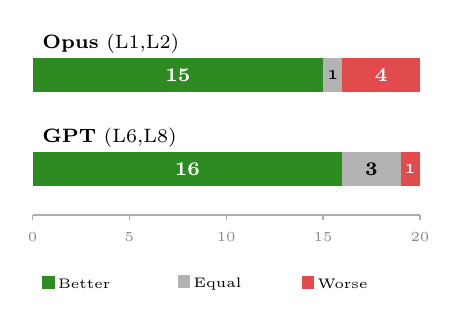
\begin{tikzpicture}[x=0.246cm,y=0.85cm]
  \path[use as bounding box] (-0.25,0) rectangle (20.25,4.18);
  % Costs relative to the original encoding; lower cost is better.
  \node[anchor=west,font=\scriptsize] at (0,3.94) {\textbf{Opus} (L1,L2)};
  \fill[vAccepted]  (0,3.22) rectangle (15,3.73);
  \fill[midgray!65] (15,3.22) rectangle (16,3.73);
  \fill[vCuts]      (16,3.22) rectangle (20,3.73);
  \node[white,font=\scriptsize\bfseries] at (7.5,3.475) {15};
  \node[black,font=\tiny\bfseries] at (15.5,3.475) {1};
  \node[white,font=\scriptsize\bfseries] at (18,3.475) {4};
  \node[anchor=west,font=\scriptsize] at (0,2.53) {\textbf{GPT} (L6,L8)};
  \fill[vAccepted]  (0,1.81) rectangle (16,2.32);
  \fill[midgray!65] (16,1.81) rectangle (19,2.32);
  \fill[vCuts]      (19,1.81) rectangle (20,2.32);
  \node[white,font=\scriptsize\bfseries] at (8,2.065) {16};
  \node[black,font=\scriptsize\bfseries] at (17.5,2.065) {3};
  \node[white,font=\tiny\bfseries] at (19.5,2.065) {1};
  % Both stacks cover the same 20 test instances.
  \draw[midgray!70,line width=0.5pt] (0,1.38) -- (20,1.38);
  \foreach \x in {0,5,10,15,20} {
    \draw[midgray!70,line width=0.5pt] (\x,1.38) -- (\x,1.30);
    \node[font=\tiny,text=midgray,anchor=north] at (\x,1.27) {\x};
  }
  \node[anchor=west,font=\tiny] at (0,0.37) {\textcolor{vAccepted}{\rule{0.16cm}{0.16cm}}\,Better};
  \node[anchor=west,font=\tiny] at (7.0,0.37) {\textcolor{midgray!65}{\rule{0.16cm}{0.16cm}}\,Equal};
  \node[anchor=west,font=\tiny] at (13.4,0.37) {\textcolor{vCuts}{\rule{0.16cm}{0.16cm}}\,Worse};
\end{tikzpicture}\par
\vspace{0.18em}
{\centering\scriptsize\color{midgray}Better means a \emph{lower} cost after 1200\,s.\par}
\end{columns}
\end{frame}

% \begin{frame}[fragile]{Still Life}
% \begin{columns}[T,onlytextwidth]
% \column{0.52\textwidth}
% \begin{lstlisting}[basicstyle=\ttfamily\scriptsize]
% % L6 (GPT-5.4) -- conjecture
% :- size(N), N>1, not lives(1,1).
% % L8 (GPT-5.4) -- symmetry breaking
% :- R = #count{ X : lives(X,1) },
%    C = #count{ Y : lives(1,Y) }, 0 < R, 0 < C, R < C.
% \end{lstlisting}
% \vspace{0.6em}
% {\footnotesize\raggedright
% Here the constraints are \alert{guesses} about optimal solutions, e.g.\ L6 requires the top-left cell to be alive. L8 is instead a true symmetry breaking: a diagonal reflection can always make the first row as full as the first column.\par}
% \vspace{0.6em}
% {\centering\scriptsize
% \setlength{\tabcolsep}{4pt}
% \begin{tabular}{@{}llcccc@{}}
% \toprule
% Enc. & Stream. & Bet. & Eq. & Wor. & Borda \\
% \midrule
% Original & --- & --- & --- & --- & 25.8 \\
% Opus 1 & L1,L2 & 15 & 1 & 4 & 56.2 \\
% Opus 2 & L2,L3 & 13 & 5 & 2 & 48.8 \\
% Opus 3 & L1,L4,L5 & 11 & 6 & 3 & 44.2 \\
% GPT 1 & L6,L7 & 10 & 5 & 5 & 50.4 \\
% \textbf{GPT 2} & \textbf{L6,L8} & \textbf{16} & \textbf{3} & \textbf{1} & \textbf{76.7} \\
% GPT 3 & L6 & 12 & 4 & 4 & 47.9 \\
% \bottomrule
% \end{tabular}\par}
% \column{0.45\textwidth}
% \centering
% \includegraphics[width=0.80\linewidth]{fig_scatter_stilllife.png}\\[0.3em]
% \footnotesize Gap to the best known cost per instance:\\ better \alert{solutions at timeout}.
% \vspace{0.8em}
% \end{columns}
% \end{frame}



\begin{frame}{Conclusions and Future Work}
\begin{columns}[T,onlytextwidth]
\column{0.5\textwidth}
\begin{itemize}
    \item Extending LLM-generated streamliners to ASP optimization requires proving optimality without losing optimal solutions.

    \item We propose an automated pipeline that generates, (empirically) validates against certified optima, and selects streamliners to accelerate optimality proofs.

    \item Experiments show PAR2 reductions up to 99.7\% on CM and 76.4\% on MC, and better solutions within the time budget on SL.
\end{itemize}
\column{0.46\textwidth}
% \begin{block}{Incorrect streamliners are still useful}
% \small The selected configurations never add stable models, so every returned cost is a \alert{valid bound}; a proof can be completed with the original encoding.
% \end{block}
\vspace{0.3em}
\textbf{Future work}
\begin{itemize}
  \item Broader range of optimization benchmarks.
  \item Structural or semantic checks on the generated rules.
  \item Repeated generations, to measure the variability across LLM runs.
\end{itemize}
\end{columns}
\end{frame}

\begin{frame}[plain]
\centering\vfill
\includegraphics[height=1.2cm]{logo_unical.png}\par\vspace{1.5em}
{\Large\bfseries Thank you!}\par\vspace{0.6em}
Questions?\par\vspace{1.5em}
{\footnotesize\color{midgray} marco.duca@unical.it \quad ilaria.frandina@gmail.com \quad francesco.ricca@unical.it}
\vfill
\end{frame}

\appendix

\begin{frame}[fragile]{Prompt used for candidate generation (abridged)}
\begin{columns}[T,onlytextwidth]
\column{0.49\textwidth}
\begin{lstlisting}[basicstyle=\ttfamily\fontsize{5.3}{6.1}\selectfont,deletecomment={[l]\%},breakatwhitespace=true,breakindent=0pt,breakautoindent=false,aboveskip=0pt]
Objective
Analyze the given ASP optimization problem in clingo and suggest 5 additional streamliner constraints to speed up reaching -- and PROVING -- the optimum.
The optimization criterion is: <criterion>.
What counts as success is the TIME to a *proved* optimum, not the time to a first good solution: clingo finds decent solutions quickly, what costs time is closing the optimality gap. A constraint is accepted when it consistently speeds up certification on the slow training instances by at least 25%; borderline wins are re-measured, and a constraint whose grounding overhead outweighs what it saves is rejected.
Current behaviour of the unmodified encoding on the training instances (certified optimum, and how long the proof took): <reference table>

Steps
(1) Analyze: read the encoding carefully. Identify what makes the optimality proof expensive: which choices are interchangeable (symmetry), which properties every optimal solution must have (implied), which partial solutions can never beat others (dominance).
(2) Design 5 unique constraints, each from a DIFFERENT family or acting on a different part of the encoding: symmetry breaking, implied constraints, dominance rules, structural bounds on the building blocks of the objective. A streamliner MAY remove optimal solutions -- the pipeline detects that and reports it back to you -- so aim for constraints that keep at least one optimal solution of every instance.
\end{lstlisting}
\column{0.49\textwidth}
\begin{lstlisting}[basicstyle=\ttfamily\fontsize{5.3}{6.1}\selectfont,deletecomment={[l]\%},breakatwhitespace=true,breakindent=0pt,breakautoindent=false,aboveskip=0pt]
(3) VERIFY before answering, one constraint at a time: does it compile in clingo 5? could it make a small instance unsatisfiable? could it remove EVERY optimal solution? is the property a THEOREM of the problem, or just a pattern of the instances shown? A numeric bound that merely happens to hold on the training instances WILL make some unseen instance unsatisfiable.
(4) Return the constraints as a JSON object {"streamliner_1": "<ASP rule>", ..., "streamliner_5": "<ASP rule>"}.

Compliance Rules
(1) Response Format: output only the JSON object; end each rule with a period.
(2) Code Quality: syntactically correct clingo 5 / ASP-Core-2; every variable bound by a positive body literal; use only predicates of the encoding or of the instance facts; do NOT redefine predicates of the encoding.
(3) Creativity: propose semantically different constraints, not syntactic variants; do not resubmit evaluated constraints; you may refine ACCEPTED ones.

Here is the ASP encoding: <encoding>
An instance looks like this (excerpt): <instance excerpt>
<from the second round: feedback on the previous candidates>
\end{lstlisting}
\end{columns}
\end{frame}

% =====================================================================
\begin{frame}[fragile]{Selected streamliners by problem}
\begin{columns}[T,onlytextwidth]
\column{0.41\textwidth}
{\footnotesize\bfseries Crossing Minimization}
\begin{lstlisting}[basicstyle=\ttfamily\tiny]
% C1 (Opus 4.8)
antecedent(N1,N2) :- in_layer(L,N1),
   in_layer(L,N2), N1 != N2, not antecedent(N2,N1),
   position(N1,_), position(N2,_).
% C2 (Opus 4.8)
:- in_layer(L,N1), in_layer(L,N2), N1 < N2,
   not antecedent(N1,N2), not antecedent(N2,N1),
   position(N1,_), position(N2,_).
% C3 (GPT-5.4)
:- in_layer(L,N1), in_layer(L,N2), N1 < N2,
   not antecedent(N1,N2), not antecedent(N2,N1).
% C4 (GPT-5.4)
:- width(0,T), in_layer(0,N0),
   #count{M: in_layer(0,M), M < N0} = 0,
   position(N0,P0), 2*P0 = T + 1, in_layer(0,N1),
   #count{M: in_layer(0,M), M < N1} = 1,
   position(N1,P1), 2*P1 > T + 1.
% C5 (GPT-5.4)
:- in_layer(L,N1), in_layer(L,N2), N1 < N2,
   position(N1,P1), position(N2,P2), P1 > P2,
   #count{M: edge(M,N1), not edge(M,N2)} = 0,
   #count{M: edge(M,N2), not edge(M,N1)} = 0,
   #count{M: edge(N1,M), not edge(N2,M)} = 0,
   #count{M: edge(N2,M), not edge(N1,M)} = 0.
\end{lstlisting}
\column{0.28\textwidth}
{\footnotesize\bfseries Maximum Clique}
\begin{lstlisting}[basicstyle=\ttfamily\tiny]
% M1 (Opus 4.8)
nonClique(X) :- clique(Y), node(X),
   X > Y, not uedge(Y,X).
% M2 (Opus 4.8)
nonClique(X) :- node(X), node(Y),
   X != Y, not edge(X,Y),
   not edge(Y,X), clique(Y), X > Y.
% M3 (GPT-5.4)
nonClique(X) | nonClique(Y) :-
   node(X), node(Y), X < Y,
   not uedge(X,Y).
% M4 (GPT-5.4)
:- nonClique(X),
   nonClique(Y) : node(Y), X != Y,
   not uedge(X,Y).
% M5 (GPT-5.4)
:- clique(Y), nonClique(X), X < Y,
   #count{Z: uedge(X,Z), Z != Y,
          not uedge(Y,Z)} = 0,
   #count{Z: uedge(Y,Z), Z != X,
          not uedge(X,Z)} = 0.
\end{lstlisting}
\column{0.29\textwidth}
{\footnotesize\bfseries Still Life}
\begin{lstlisting}[basicstyle=\ttfamily\tiny]
% L1 (Opus 4.8)
lives(1,1) :- size(N), value(1).
% L2 (Opus 4.8)
lives(1,N) :- size(N), value(N),
   value(1).
% L3 (Opus 4.8)
:- lives(X,Y), lives(X+1,Y),
   lives(X,Y+1), lives(X+1,Y+1),
   value(X), value(Y),
   value(X+1), value(Y+1).
% L4 (Opus 4.8)
:- lives(1,1), lives(2,2),
   not lives(1,2), not lives(2,1).
% L5 (Opus 4.8)
lives(1,2) :- size(N), value(2),
   lives(1,1).
% L6 (GPT-5.4)
:- size(N), N>1, not lives(1,1).
% L7 (GPT-5.4)
:- size(N), N>1,
   1 = #count { X : lives(X,1) }.
% L8 (GPT-5.4)
:- R = #count { X : lives(X,1) },
   C = #count { Y : lives(1,Y) },
   0 < R, 0 < C, R < C.
\end{lstlisting}
\end{columns}
\end{frame}

\begin{frame}[fragile]{Still Life}
\begin{tabular}{@{}llcccc@{}}
\toprule
Enc. & Stream. & Bet. & Eq. & Wor. & Borda \\
\midrule
Original & --- & --- & --- & --- & 25.8 \\
Opus 1 & L1,L2 & 15 & 1 & 4 & 56.2 \\
Opus 2 & L2,L3 & 13 & 5 & 2 & 48.8 \\
Opus 3 & L1,L4,L5 & 11 & 6 & 3 & 44.2 \\
GPT 1 & L6,L7 & 10 & 5 & 5 & 50.4 \\
\textbf{GPT 2} & \textbf{L6,L8} & \textbf{16} & \textbf{3} & \textbf{1} & \textbf{76.7} \\
GPT 3 & L6 & 12 & 4 & 4 & 47.9 \\
\bottomrule
\end{tabular}
\centering
\begin{block}{Why Borda?}
{\scriptsize\raggedright
No optimum is certified for $n=11$--$30$ in 1200\,s:
compare the \emph{best cost found}. Per instance: \textbf{1 pt} per worse rival, \textbf{$\frac12$ pt} per tie (6 rivals). Scale to \textbf{0--100}. \textbf{Higher} means better relative costs across all \textbf{7 encodings}.
\par}
\end{block}
\end{frame}

\end{document}